
\begin{figure}[H]
    \centering
    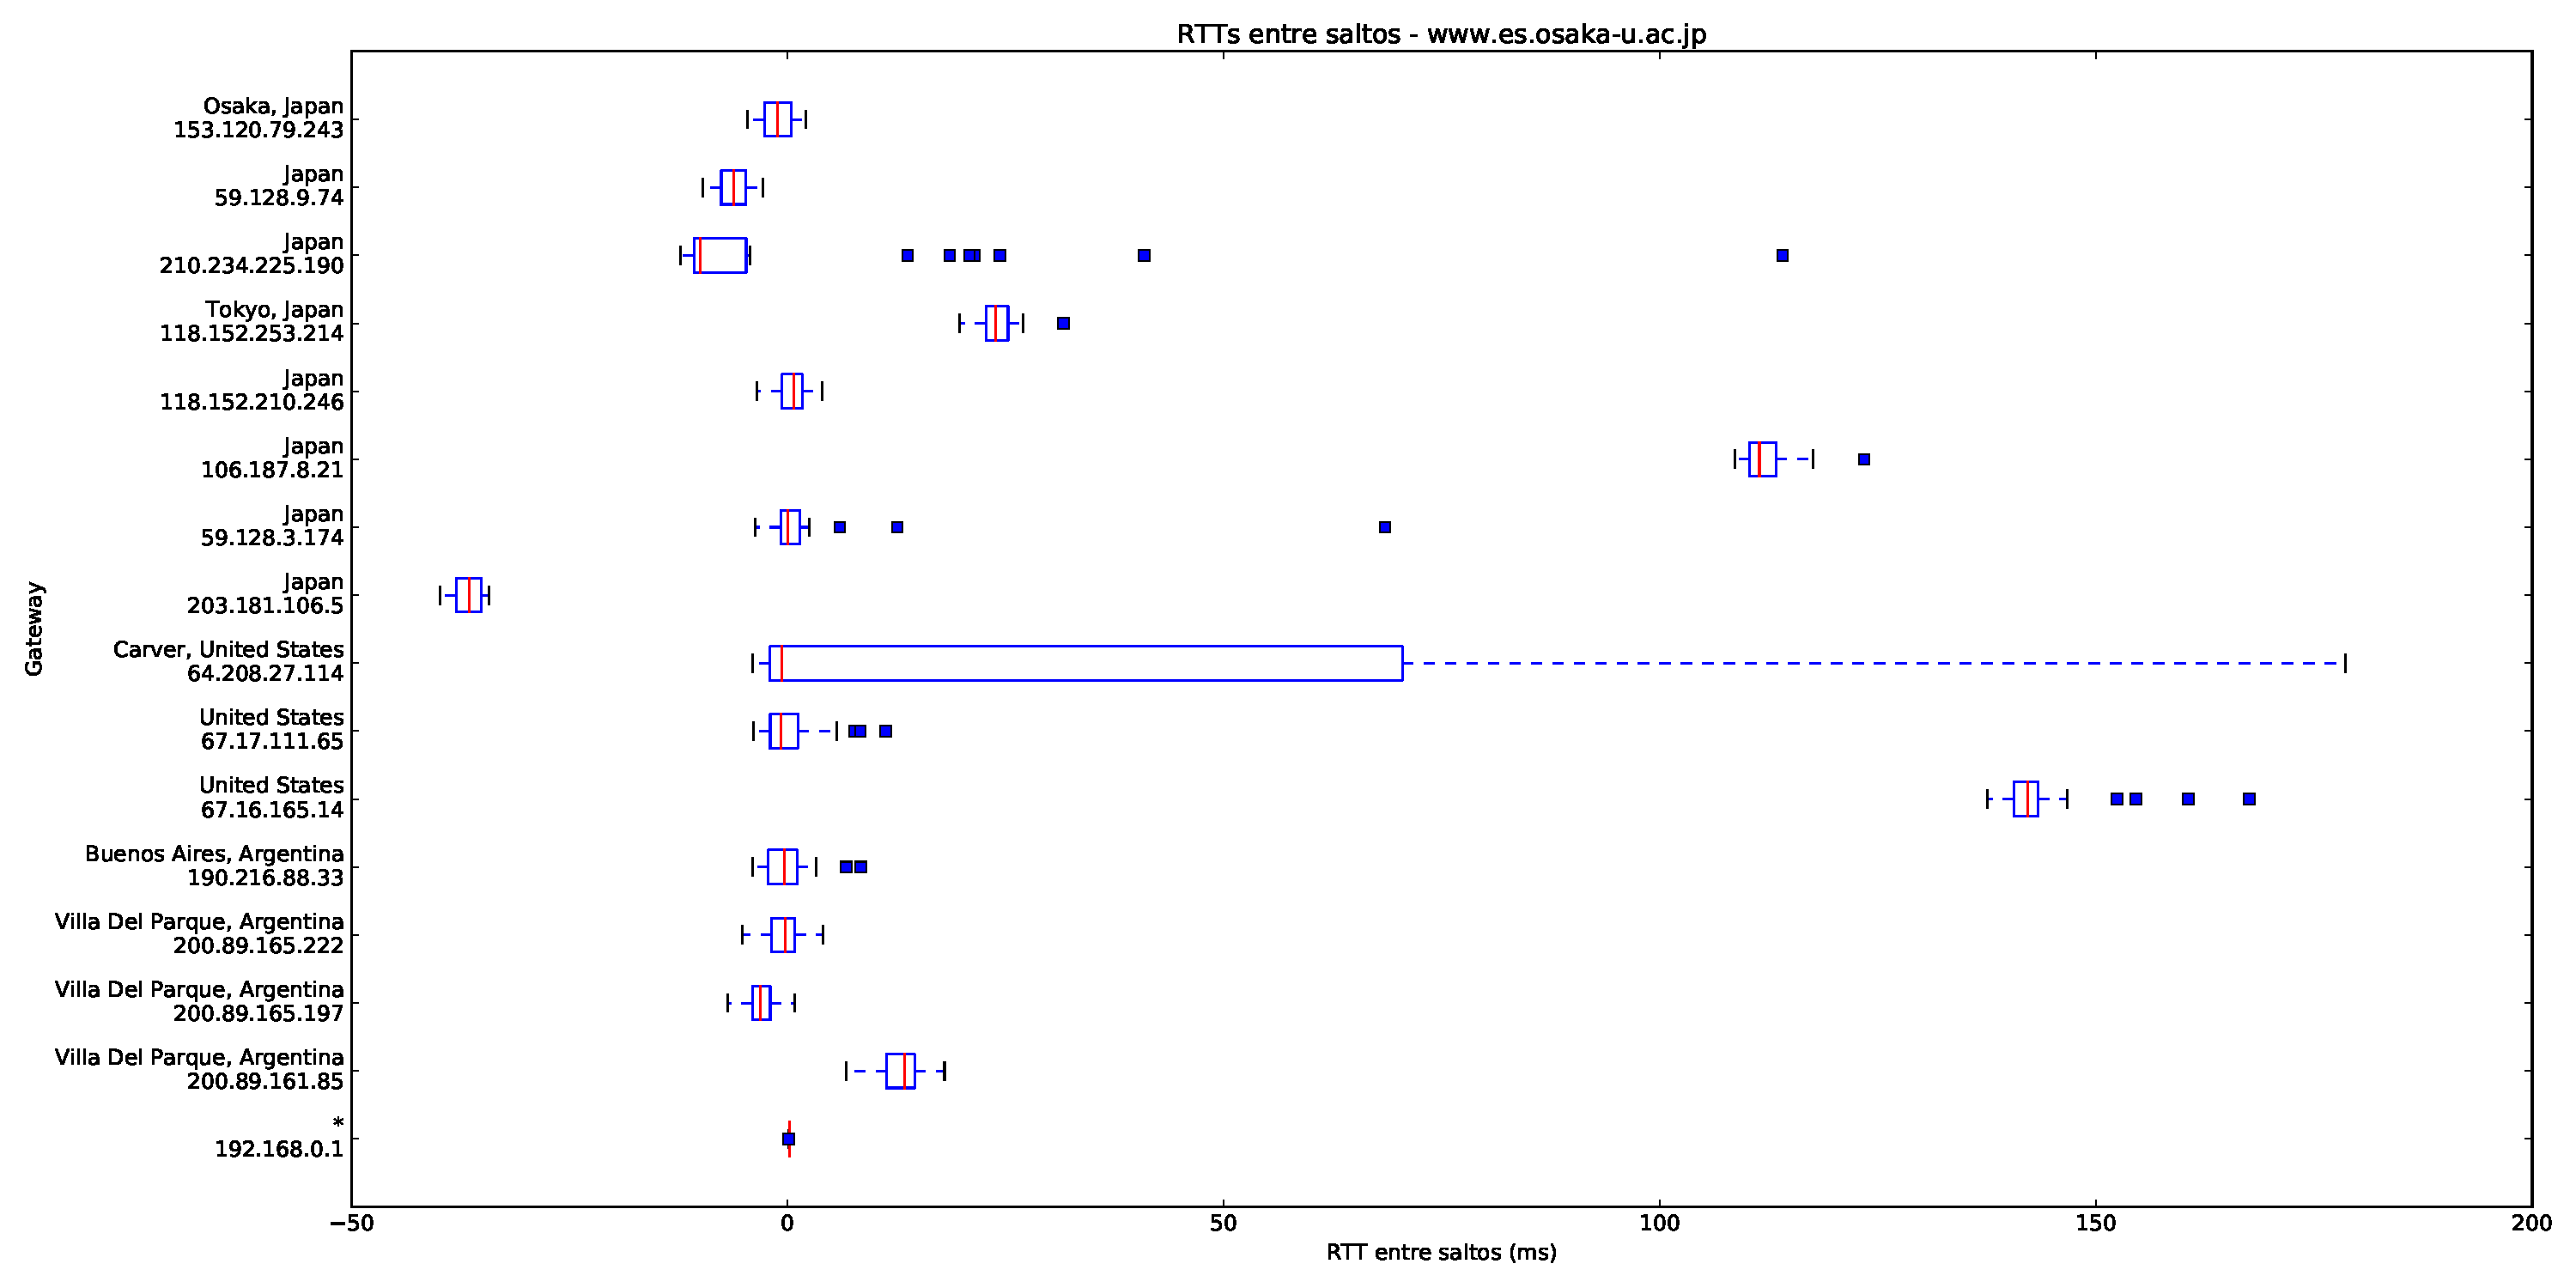
\includegraphics[width=8.5cm]{img/grafico1-www-es-osaka-u-ac-jp.pdf}
    \caption{\normalfont RTTs entre saltos. El valor asignado al $i$-ésimo nodo corresponde al salto entre el $i$-ésimo y el $i - 1$-ésimo nodo. Para el primer nodo se utiliza simplemente su RTT.}
\end{figure}

\begin{figure}[H]
    \centering
    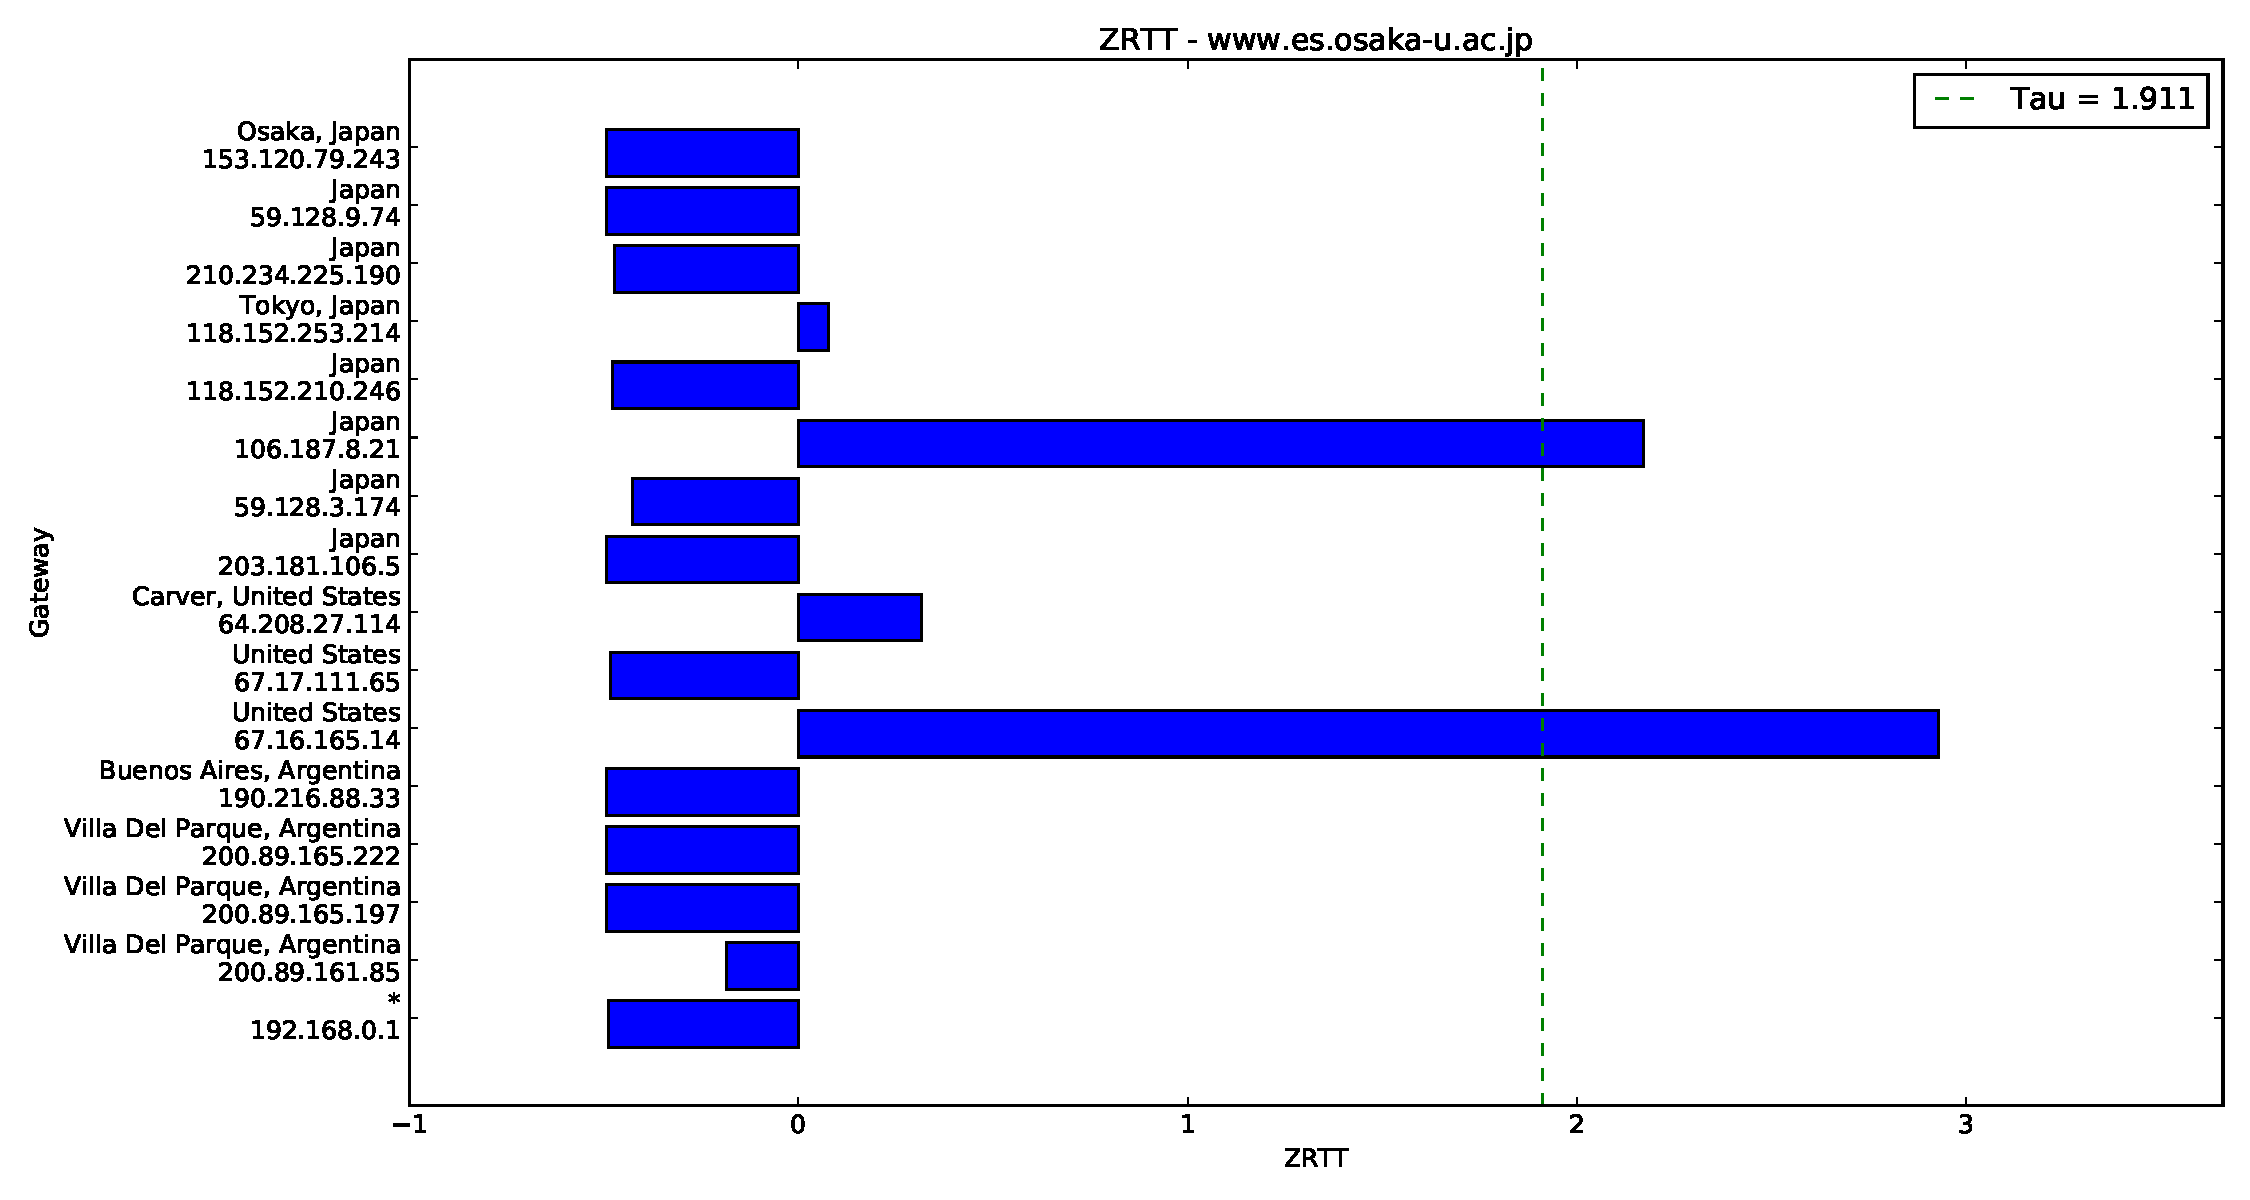
\includegraphics[width=8.5cm]{img/grafico2-www-es-osaka-u-ac-jp.pdf}
    \caption{\normalfont ZRTTs entre saltos.}
\end{figure}

\begin{figure}[H]
    \centering
    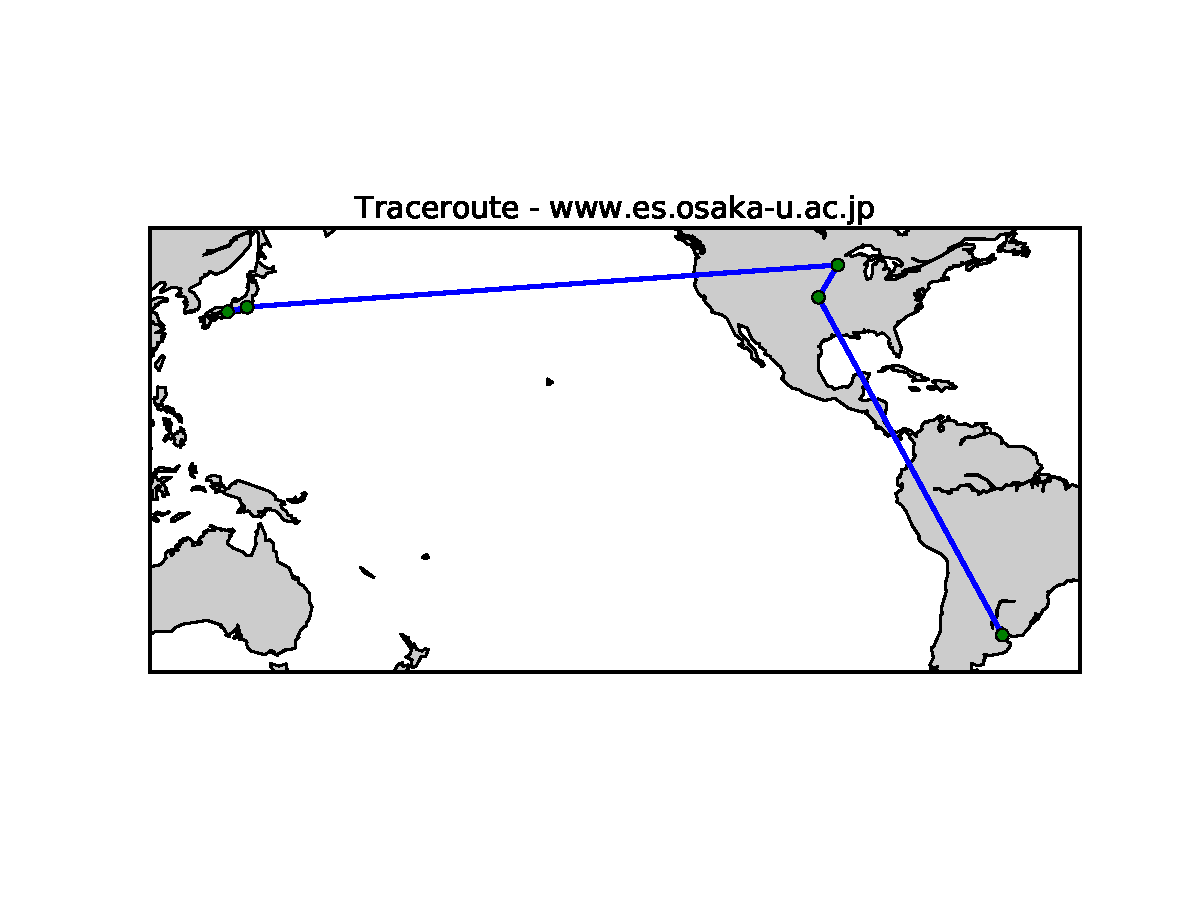
\includegraphics[width=8.5cm]{img/grafico3-www-es-osaka-u-ac-jp.pdf}
    \caption{\normalfont Ubicación geográfica estimada de la ruta tomada.}
\end{figure}
